\newpage
\section{New use cases}

\subsection{Actors}

\paragraph{}
From the previous reflection on lifecycle, a few new use cases and functions are raised.

\paragraph{}
First, there are new actors, so if we recap and define all of them:

\begin{itemize}
    \item \textbf{Developers} are the people that use the system to store and retrieve files. They are authenticated and authorized by the system.
    \item \textbf{Repo administrator} is the people or external system who defines the repositories and the authorizations
    \item \textbf{System administrator} is someone managing the system and its resources. He is owner of the system and defines the system configuration. He maintains and deploy the system.
    \item \textbf{Unauthorized user} is anyone unknown of the system
\end{itemize}

\subsection{Use cases}

\paragraph{}
The repo administrator has access to a few more use cases:

\begin{figure}[h]
    \centering
    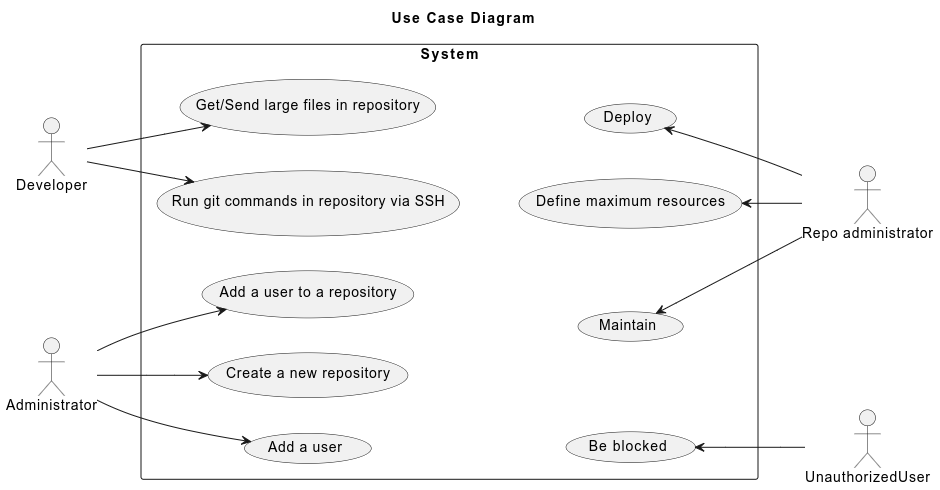
\includegraphics[width=\textwidth]{iteration_01/diagrams/admin_use_cases.png}
    \caption{Updated use cases of the system}
    \label{fig:admin_use_cases}
\end{figure}

\newpage
\subsection{What does it change?}

\paragraph{}
The system will have to expose not only the git api and the git lfs api (ports 22 and 80), but also a secured SSH access to the whole system to the admin, so we might expand the first function \textbf{F1} to include \textbf{F1.5}: Handle administrator SSH access. 

\paragraph{}
A new function \textbf{F7} might be introduced: "Manage the system" which will include the following sub-functions:

\begin{figure}[h]
    \centering
    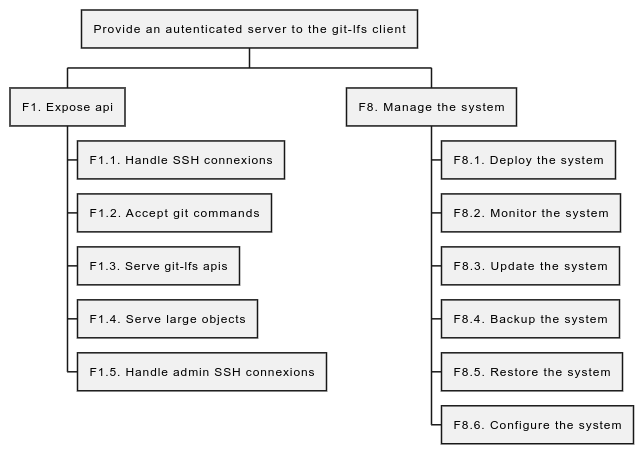
\includegraphics[width=0.8\textwidth]{iteration_01/diagrams/functions_v2.png}
    \caption{Manage the system}
    \label{fig:functions_v2}
\end{figure}

\newpage
\subsection{New components}

\paragraph{}
The administration use cases lead to introduce a few more components. As much as possible, to make deployments easier, minimal access should be used to go inside containers. Logs should be available from inside the system, but outside the containers. 

\paragraph{}
The configuration is done also outside of the container, if possible during deployment, so the next deployment do not need to require a new configuration step.

\paragraph{}
Backups system should also be implemented on the storage containers (lfs, repo, databases). 

The figure \ref{fig:components_v2} shows the new components for these use cases. 

\begin{figure}[ht]
    \centering
    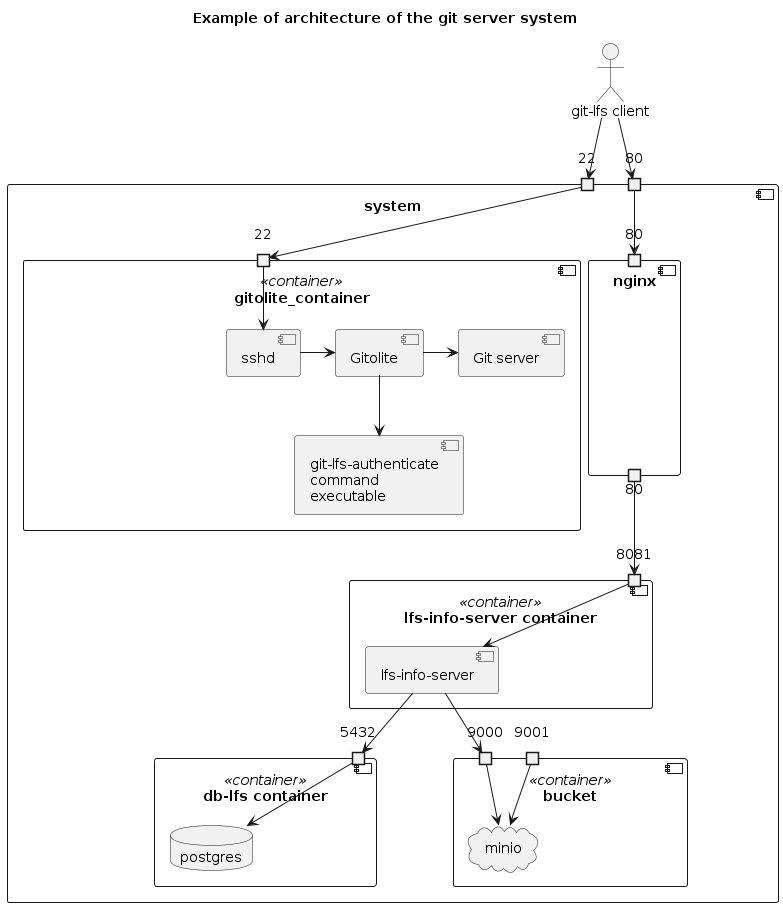
\includegraphics[width=\textwidth]{iteration_01/diagrams/components.png}
    \caption{Updated components}
    \label{fig:components_v2}
\end{figure}

